\begin{figure*}[!t]
\centering
% Fig. 1: ArtiGate-YOLO overview (top) and the AGA block (bottom). TikZ, no external files.
\begin{tikzpicture}[
  font=\scriptsize,
  >={Stealth[length=1.6mm]},
  blk/.style={draw, rounded corners=1.5pt, minimum height=6mm, minimum width=11mm, align=center, fill=white},
  bb/.style={blk, fill=gray!10},
  new/.style={blk, fill=orange!18, draw=orange!70!black, thick},
  head/.style={blk, fill=blue!8},
  map/.style={draw=orange!70!black, fill=orange!8, minimum size=5mm, inner sep=0pt},
  lab/.style={font=\tiny, text=black!70},
  line/.style={->, thick, black!70},
  aline/.style={->, thick, orange!70!black, dashed},
]
% ---------------------------------------------------------------- backbone row
\node[bb] (in) {RGB\\$640^2$};
\node[bb, right=3mm of in] (c0) {Conv$\times$2\\C3k2};
\node[lab, anchor=north west] at ($(c0.south)+(0.7mm,0)$) {B2, $s{=}4$};
\node[new, right=5mm of c0] (aga2) {AGA};
\node[bb, right=3mm of aga2] (c1) {Conv\\C3k2};
\node[lab, below=0mm of c1] {B3, $s{=}8$};
\node[new, right=3mm of c1] (aga3) {AGA};
\node[bb, right=3mm of aga3] (c2) {Conv, C3k2,\\SPPF, C2PSA};
\node[lab, below=0mm of c2] {P4, P5};
\node[head, right=4mm of c2] (neck) {PAN neck\\P2--P5};
\node[head, right=3mm of neck] (seg) {Segment26\\boxes P2--P5\\protos P3--P5};
\draw[line] (in) -- (c0);
\draw[line] (c0) -- (aga2);
\draw[line] (aga2) -- (c1);
\draw[line] (c1) -- (aga3);
\draw[line] (aga3) -- (c2);
\draw[line] (c2) -- (neck);
\draw[line] (neck) -- (seg);
\draw[line] (aga2.north) -- ++(0,3mm) -| ($(neck.north)+(-3mm,0)$);
\draw[line] (aga3.north) -- ++(0,1.5mm) -| ($(neck.north)+(0mm,0)$);
% ---------------------------------------------------------------- artifact head
\node[new, below=9mm of c0] (ah) {Artifact head\\$1{\times}1$, $3{\times}3$, $3{\times}3$, $1{\times}1$};
\draw[line] (c0.south) -- (ah.north);
\node[map, right=6mm of ah, label={[lab]below:hair}] (m1) {};
\node[map, right=1mm of m1, label={[lab]below:ruler}] (m2) {};
\node[map, right=1mm of m2, label={[lab]below:ink}] (m3) {};
\node[map, right=1mm of m3, label={[lab]below:corner}] (m4) {};
\node[fit=(m1)(m4), inner sep=1pt] (maps) {};
\draw[line] (ah) -- (m1);
\node[blk, right=5mm of m4, minimum width=9mm] (amax) {$\max_k$\\$\bar{A}$};
\draw[line] (m4) -- (amax);
\draw[aline] (amax.north) |- ($(aga2.south)+(0,-4.5mm)$) -- (aga2.south);
\draw[aline] (amax.north) |- ($(aga3.south)+(0,-4.5mm)$) -- (aga3.south);
\node[lab, align=left, right=3mm of amax] (loss) {$\mathcal{L}_{\mathrm{art}}$: BCE + Dice on\\labelled cells (synthetic\\masks, flags, rules)};
\draw[->, thick, blue!60!black] ($(m4.south)+(0,-2.5mm)$) -- ++(0,-2mm) -| (loss.south);
\end{tikzpicture}

\vspace{2mm}
\begin{tikzpicture}[
  font=\scriptsize,
  >={Stealth[length=1.6mm]},
  blk/.style={draw, rounded corners=1.5pt, minimum height=6mm, align=center, fill=white},
  op/.style={draw, circle, inner sep=0.5pt, minimum size=4.5mm},
  line/.style={->, thick, black!70},
  aline/.style={->, thick, orange!70!black, dashed},
]
\node (F) {$F$};
\node[blk, right=3mm of F] (ca) {Channel attention\\(shared with CBAM)};
\node[blk, right=4mm of ca] (pool) {$[\mathrm{Avg}_C F';\ \mathrm{Max}_C F';\ \bar{A}]$};
\node[blk, right=3mm of pool] (conv) {conv $7{\times}7$\\$\sigma$};
\node[op, right=3mm of conv] (mul1) {$\odot$};
\node[op, right=6mm of mul1] (mul2) {$\odot$};
\node[right=3mm of mul2] (out) {$F''$};
\node[blk, below=4mm of mul2, fill=orange!8, draw=orange!70!black] (gate) {$\max(0,\,1-\beta\bar{A})$};
\node[below=5mm of pool, text=orange!70!black] (A) {$\bar{A}$ (resized by max pooling)};
\draw[line] (F) -- (ca);
\draw[line] (ca) -- node[above, font=\tiny]{$F'$} (pool);
\draw[line] (pool) -- (conv);
\draw[line] (conv) -- (mul1);
\draw[line] (mul1) -- (mul2);
\draw[line] (mul2) -- (out);
\draw[line] (ca.north) -- ++(0,3mm) -| (mul1.north);
\draw[aline] (A.north) -- (pool.south);
\draw[aline] (A.east) -| (gate.west) ;
\draw[line] (gate) -- (mul2);
\end{tikzpicture}

\caption{ArtiGate-YOLO. Top: the artifact head reads the stride-4 backbone feature B2 and predicts four artifact maps; their pixel-wise maximum $\bar{A}$ is passed to the two AGA blocks that replace CBAM after B2 and B3. The rest is YOLO26n-seg with a P2 detection level; mask prototypes are built from P3--P5 at stride~4. Bottom: the AGA block. Its channel attention is the CBAM channel attention; the spatial attention receives $\bar{A}$ as a third input and the output is multiplied by $\max(0,1-\beta\bar{A})$. The weights on $\bar{A}$ and $\beta$ start at zero, so AGA equals CBAM at initialization. Dashed: artifact map; by default it is detached, so the segmentation loss does not train the artifact head.}
\label{fig:overview}
\end{figure*}

\subsection{Base Network}
The base network is YOLO26n-seg~\cite{jocher2026yolo26} with an additional P2 output, so boxes and mask coefficients are predicted at strides 4, 8, 16 and 32. Mask prototypes are computed from P3--P5 and upsampled once, which keeps them at stride~4. The CBAM baseline of our conference paper~\cite{iceeis2026own} (row A1 in Section~\ref{sec:protocol}) inserts CBAM~\cite{woo2018cbam} directly after the stride-4 feature B2 and the stride-8 feature B3 of the backbone. ArtiGate-YOLO keeps this network and replaces the two CBAM blocks with AGA blocks fed by an artifact head (Fig.~\ref{fig:overview}).

\subsection{Artifact Head}
Let $B_2\in\mathbb{R}^{C_2\times H/4\times W/4}$ be the B2 feature map ($C_2=64$ at scale n). The artifact head reduces it with a $1\times1$ convolution to $c_h=32$ channels, refines it with two $3\times3$ convolutions (these three convolutions are each followed by batch normalization and SiLU) and maps it with a plain $1\times1$ convolution to $K=4$ logits $Z\in\mathbb{R}^{K\times H/4\times W/4}$ for hair, ruler, marker ink and dark corner. The artifact probabilities are $A_k=\sigma(Z_k)$. The bias of the last layer is initialized to $\log(\pi/(1-\pi))$ with $\pi=0.01$ because artifacts cover few pixels. The combined map is the pixel-wise maximum over types,
\begin{equation}
\bar{A}=\max_{k=1,\dots,K} A_k ,
\label{eq:abar}
\end{equation}
computed from detached logits by default, so that the segmentation loss cannot push the head towards maps that hide the lesion; the head is then trained only by its own loss (Section~\ref{sec:loss}). Together with the two AGA blocks, the head adds about 21 thousand parameters (0.8\% of the deployed model) and 1.05~GFLOPs at $640\times640$ input (Supplementary Section~S10).

\subsection{Artifact-Gated Attention}
Given a feature map $F\in\mathbb{R}^{C\times H'\times W'}$ at the position of a CBAM block, AGA first applies the CBAM channel attention,
\begin{equation}
F'=\sigma\big(\mathrm{MLP}(\mathrm{Avg}_{HW}F)+\mathrm{MLP}(\mathrm{Max}_{HW}F)\big)\odot F,
\label{eq:ca}
\end{equation}
with a shared two-layer MLP (reduction 16, no bias). The artifact map is resized to $H'\times W'$ by max pooling, which keeps thin hairs visible at stride 8, giving $\bar{A}'$. The spatial attention and the gate are
\begin{equation}
\begin{aligned}
F''={}&F'\odot\sigma\Big(f^{7\times7}\big([\mathrm{Avg}_C F';\,\mathrm{Max}_C F';\,\bar{A}']\big)\Big)\\
&\odot\max\big(0,\,1-\beta\bar{A}'\big),
\end{aligned}
\label{eq:aga}
\end{equation}
where $f^{7\times7}$ is a $7\times7$ convolution with three input channels and $\beta$ is a learned scalar. The weights of $f^{7\times7}$ on the $\bar{A}'$ channel and $\beta$ are initialized to zero, so at initialization \eqref{eq:aga} reduces exactly to CBAM, and AGA departs from CBAM only as far as training moves these parameters away from zero. $\beta$ is not clamped: with a clamp to $[0,1]$, a $\beta$ that drifts below zero receives no gradient and stays there, which we observed in a development run. A positive $\beta$ attenuates features where artifacts are predicted and a negative $\beta$ would amplify them; weight decay pulls $\beta$ towards zero, that is, towards CBAM. We report the learned $\beta$ of each block.

\subsection{Training Targets Without Manual Annotation}\label{sec:targets}
\paragraph{Synthetic artifacts}
During training, each image receives procedurally drawn artifacts with probability $p_{\mathrm{synth}}=0.7$. Each of the four types is drawn independently (probabilities 0.5 for hair and 0.3 for the others, at least one type per image) with a severity sampled uniformly from $\{1,2,3,4\}$. Hair strands are cubic B\'ezier curves of random length, curvature, width and colour; rulers are light (occasionally dark) bands with tick marks and numerals along one image border, or two borders at the highest severity; marker ink forms dots, arcs or strokes around the lesion in purple, blue or black; dark corners are a circular dermatoscope aperture with a soft edge. The drawing order follows the physical layering (ink, hair, ruler, aperture). Rulers and marks never overlap the lesion bounding box and the aperture always contains it; only hair may cross the lesion, whose mask is unchanged. Every drawn artifact yields an exact mask, and the anti-aliased edge around it is marked as unknown; a later layer can cover an earlier one (for example, the aperture over hair), and the earlier mask is kept. Artifacts are drawn inside the image content area only, never on letterbox padding. The full parameter table is in Supplementary Section~S3, and examples are shown in Fig.~\ref{fig:synthetic}.

\paragraph{Partial labels}
For each artifact type a pixel is \emph{present}, \emph{absent} or \emph{unknown}. Synthetic artifacts give present pixels. Absent pixels come from two sources: image-level labels of the ISIC 2018 training images~\cite{bissoto2020debiasing,bissoto2022artifact}, which mark every pixel of an image as absent for the types it does not contain, and conservative rules that only exclude pixels which cannot show the artifact (for example, no hair where the morphological black-hat response is low, no dark corner where the brightness is at least 70; Supplementary Section~S4). All remaining pixels are unknown and do not contribute to the loss. Without the absent pixels the head would admit the trivial solution of predicting artifacts everywhere.

\paragraph{Joint augmentation}
The four target maps are stored as extra image channels (255 present, 0 absent, 114 unknown) and pass through the standard Ultralytics augmentation together with the image: mosaic, rotation, scaling, flips, mix-up and copy-paste. The maps therefore stay aligned with the image without changes to the augmentation code; after interpolation, a value of at least $0.75\cdot255$ counts as present, a value of at most $0.1\cdot255$ as absent and anything in between as unknown, so that mix-up of an absent with an unknown pixel stays unknown, and padding added by the augmentations is coded as unknown or absent, both correct because padding contains no artifact. Colour augmentation is applied to the image channels only, and the maps are split off before the forward pass.

\begin{figure*}[!t]
\centering
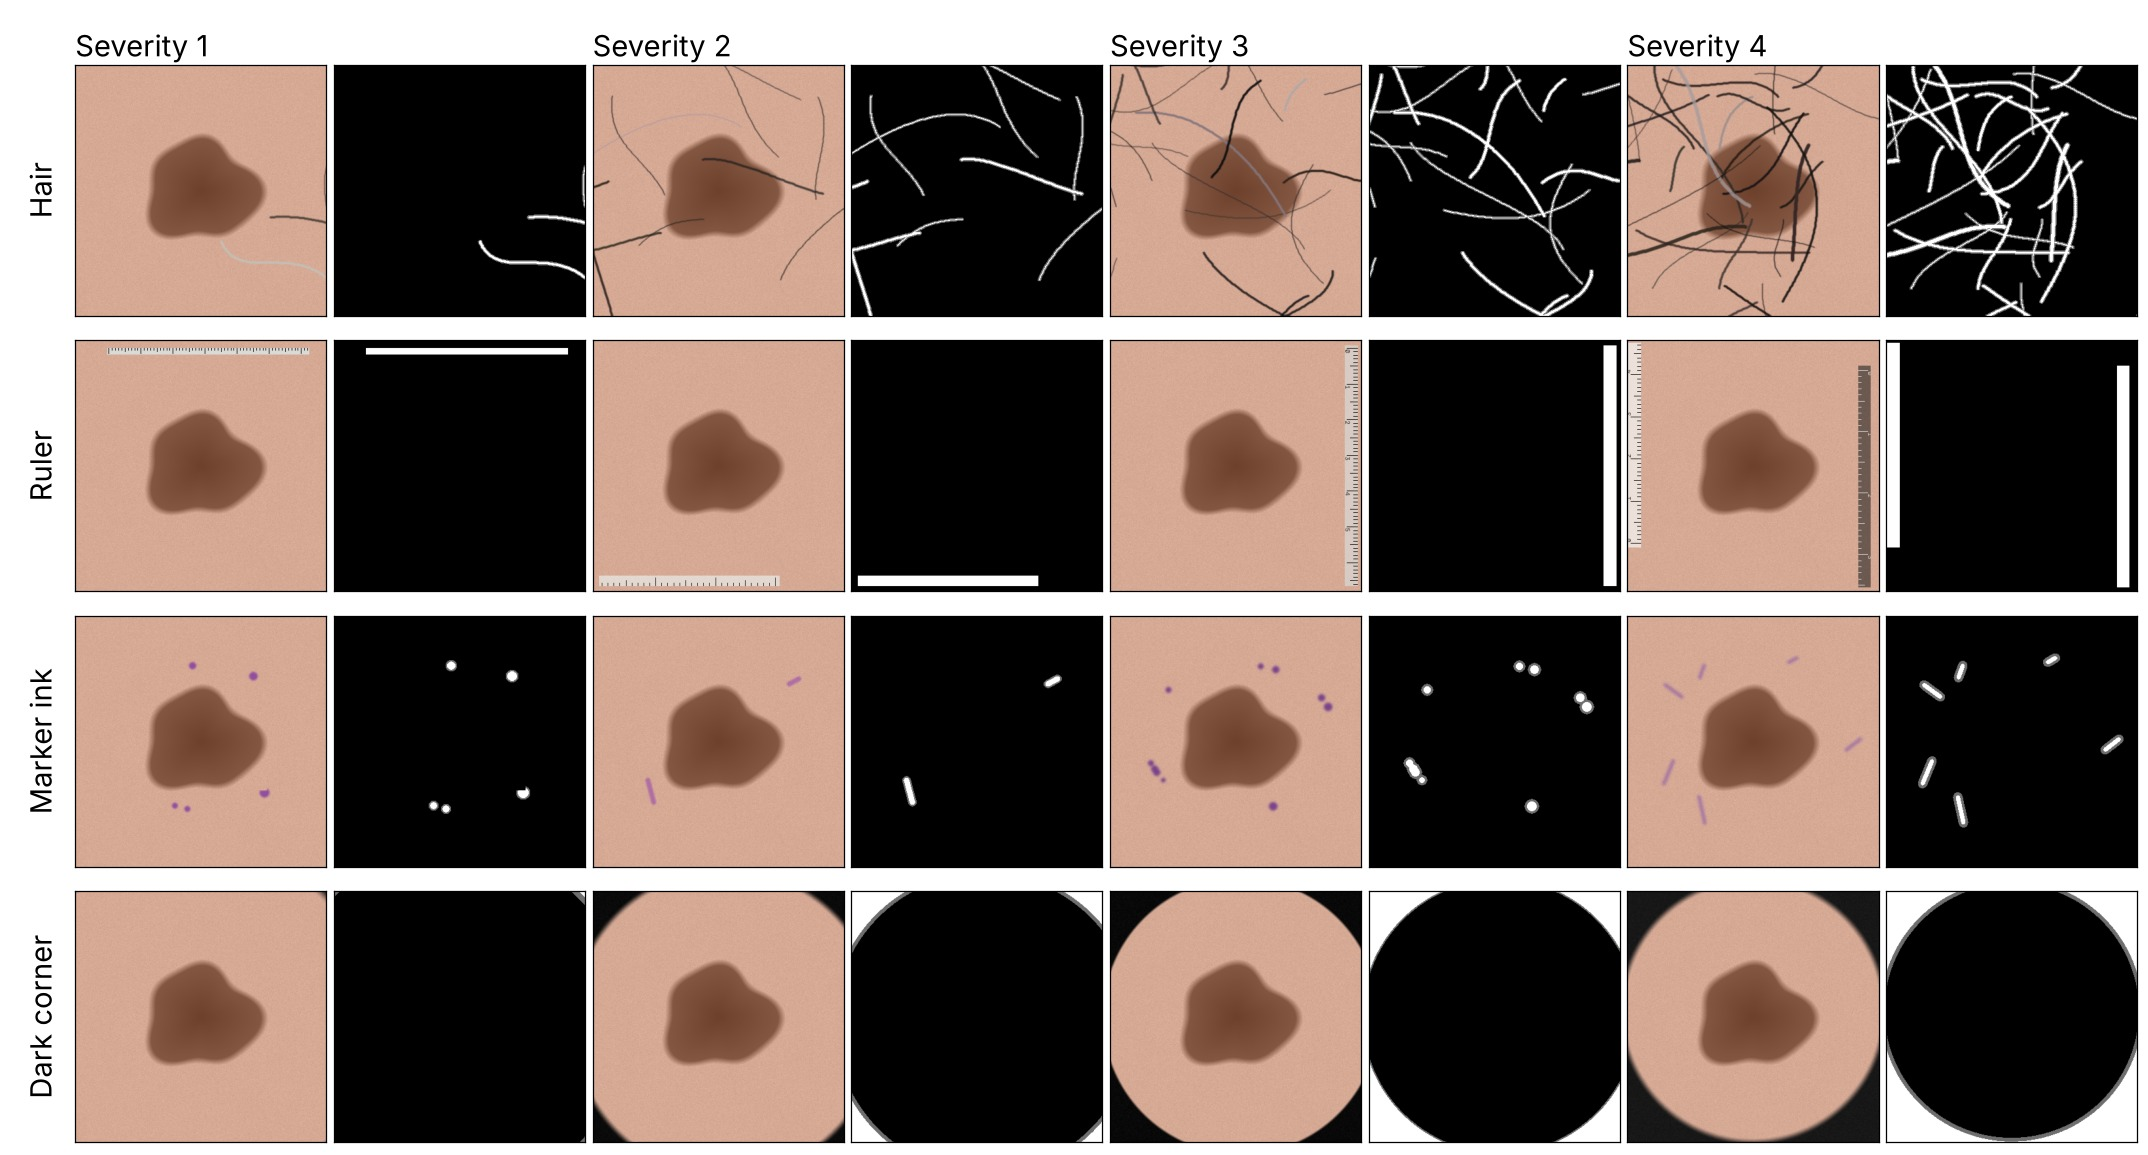
\includegraphics[width=\textwidth]{figures/synthetic_artifacts.jpg}
\caption{Procedural artifacts at severities 1--4 for hair, ruler, marker ink and dark corner (rows). Each severity shows the image and the training target of that type: white, present; grey, pixels changed by the artifact but outside its label (unknown); black, not changed by the generator (absent or unknown, depending on the image-level labels and rules). At severity~1 the aperture often stays outside the image because it must contain the lesion. \TBD{Placeholder rendered on a drawn lesion; regenerate on an ISIC 2018 training image with scripts/figure\_synthetic\_artifacts.py before submission.}}
\label{fig:synthetic}
\end{figure*}

\subsection{Loss}\label{sec:loss}
The artifact head is supervised at its own resolution (stride~4). A target cell is positive if any pixel inside it is present, negative if every pixel inside it is absent, and ignored otherwise; this keeps one-pixel hairs as positives after downsampling. Let $t_{k,i}\in\{0,1\}$ be the target and $w_{k,i}\in\{0,1\}$ the label mask of cell $i$ for type $k$, and $\mathcal{K}$ the set of types with at least one labelled cell in the batch. The artifact loss is
\begin{equation}
\mathcal{L}_{\mathrm{art}}=\frac{1}{|\mathcal{K}|}\sum_{k\in\mathcal{K}}\Big(\mathcal{L}^{k}_{\mathrm{BCE}}+1-\frac{2\sum_i w_{k,i}A_{k,i}t_{k,i}+1}{\sum_i w_{k,i}A_{k,i}+\sum_i w_{k,i}t_{k,i}+1}\Big),
\label{eq:artloss}
\end{equation}
where $\mathcal{L}^{k}_{\mathrm{BCE}}$ is the binary cross-entropy averaged over the labelled cells of type $k$ and the second term is a soft Dice loss~\cite{milletari2016vnet} over the same cells; sums run over all cells in the batch. The total loss is
\begin{equation}
\mathcal{L}=\mathcal{L}_{\mathrm{seg}}+\lambda\,\mathcal{L}_{\mathrm{art}},\qquad\lambda=1,
\label{eq:total}
\end{equation}
where $\mathcal{L}_{\mathrm{seg}}$ is the unchanged end-to-end YOLO26 segmentation loss (box overlap and box distance, mask, classification and semantic-mask terms for its one-to-many and one-to-one assignments). Models without an artifact head are trained with $\mathcal{L}_{\mathrm{seg}}$ alone by the same code.

\subsection{Inference}
At inference ArtiGate-YOLO takes one RGB image with no preprocessing. The artifact maps are a by-product that can be displayed with the lesion mask (Fig.~\ref{fig:qualitative}).
